\section{Что такое исследования?}

Проведение исследований неразрывно связано с понятиями - данные, информация, знания. Эти термины всем знакомы и кажутся самодостаточными и очевидными. Их определения и различные трактовки можно легко найти в интернете, например на википедии.



\marginpar{
        \url{https://ru.wikipedia.org/wiki/информация} 
        
\includegraphics[scale=0.5]{pics/qr_wikipedia_information.png} 
        \newline
        \url{https://ru.wikipedia.org/wiki/данные} 
        
\includegraphics[scale=0.5]{pics/qr_wikipedia_data.png}}

Но приведем здесь одну из интерпретаций, которую будет в дальнейшем придерживаться. Можно нарисовать следующую схему, показывающую связь между данными и информацией.  

\begin{figure}[h!]
	\begin{center}
		

\tikzset{every picture/.style={line width=0.75pt}} %set default line width to 0.75pt        

\begin{tikzpicture}[x=0.75pt,y=0.75pt,yscale=-1,xscale=1]
%uncomment if require: \path (0,239); %set diagram left start at 0, and has height of 239

%Rounded Rect [id:dp8355723819738923] 
\draw [fill={rgb, 255:red, 184; green, 233; blue, 134 }  ,fill opacity=1 ]  (98,119.5) .. controls (98,115.08) and (101.58,111.5) .. (106,111.5) -- (202.97,111.5) .. controls (207.39,111.5) and (210.97,115.08) .. (210.97,119.5) -- (210.97,143.5) .. controls (210.97,147.92) and (207.39,151.5) .. (202.97,151.5) -- (106,151.5) .. controls (101.58,151.5) and (98,147.92) .. (98,143.5) -- cycle ;
%Rounded Rect [id:dp6680308810096447] 
\draw [fill={rgb, 255:red, 184; green, 233; blue, 134 }  ,fill opacity=1 ]  (270,119.5) .. controls (270,115.08) and (273.58,111.5) .. (278,111.5) -- (374.97,111.5) .. controls (379.39,111.5) and (382.97,115.08) .. (382.97,119.5) -- (382.97,143.5) .. controls (382.97,147.92) and (379.39,151.5) .. (374.97,151.5) -- (278,151.5) .. controls (273.58,151.5) and (270,147.92) .. (270,143.5) -- cycle ;
%Straight Lines [id:da6784338312341602] 
\draw    (211,131) -- (268,131) ;
\draw [shift={(268,131)}, rotate = 180] [color={rgb, 255:red, 0; green, 0; blue, 0 }  ][line width=0.75]    (10.93,-3.29) .. controls (6.95,-1.4) and (3.31,-0.3) .. (0,0) .. controls (3.31,0.3) and (6.95,1.4) .. (10.93,3.29)   ;

% Text Node
\draw (127,125) node [anchor=north west][inner sep=0.75pt]   [align=left] {Данные};
% Text Node
\draw (286,125) node [anchor=north west][inner sep=0.75pt]   [align=left] {Информация};

% Text Node
\draw (90,160) node [anchor=north west][inner sep=0.75pt]   [align=left] {То, что зафиксировано};
% Text Node
\draw (272,160) node [anchor=north west][inner sep=0.75pt]   [align=left] {То, что обработано};


\end{tikzpicture}

		\caption{Связь данных и информации}
		\label{ris:data_info_chart_1}
	\end{center}
\end{figure}

Под данными мы будем понимать значения каких-то параметров или фактов записанных на определенном носителе. Данные - это совокупность сведений, зафиксированных на определенном носителе в форме пригодной для постоянного хранения обработки и интерпретации. Например замеры давления на приеме УЭЦН записанные в базу данных - это данные. Главное, что они записаны и к ним можно получить доступ при необходимости. 
Информация - это результат преобразования и анализа данных направленный на практическую деятельность -- на принятие решений. Хотя информация должна обрести некоторую форму представления, то есть превратиться в данные, чтобы ей можно было обмениваться, информация есть в первую очередь интерпретация (смысл) такого представления. Информация всегда привязана к практической деятельности. Без применения информация превращается в данные. 

В инженерной практике - часто используют понятие принятия решений для обозначения практической деятельности. И мы будем использовать его в данном пособии подразумевая под решением какое то действие связанное с необратимой тратой ресурсов - времени, материалов, денег для реализации практической деятельности. Мы будет считать что решения связаны с результатами, которые можно оценить тем или иным способом (хотя это и не всегда так). Например решением может быть решение о проведении ГТМ, строительстве скважины, выборе типа оборудования для спуска в скважину, решении о проведении исследования. В связи с ограниченностью ресурсов не все решения могут быть реализованы на практике, поэтому задача принятия решений является актуальной.

\marginpar{Задачу экономической теории можно сформулировать как задачу о трате ограниченных ресурсов для решения практически значимых задач, поищите определения в интернете или литературе.}

Цепочку связи данных, информации и принятия решений можно показать на следующей схеме как на рисунке \ref{ris:data_info_decision_chart_1}. 

\begin{figure}[h!]
	\begin{center}
		

\tikzset{every picture/.style={line width=0.75pt}} %set default line width to 0.75pt        

\begin{tikzpicture}[x=0.75pt,y=0.75pt,yscale=-1,xscale=1]
%uncomment if require: \path (0,300); %set diagram left start at 0, and has height of 300

%Rounded Rect [id:dp2235462280724534] 
\draw  [fill={rgb, 255:red, 184; green, 233; blue, 134 }  ,fill opacity=1 ] (135.2,68) .. controls (135.2,63.58) and (138.78,60) .. (143.2,60) -- (227.97,60) .. controls (232.39,60) and (235.97,63.58) .. (235.97,68) -- (235.97,92) .. controls (235.97,96.42) and (232.39,100) .. (227.97,100) -- (143.2,100) .. controls (138.78,100) and (135.2,96.42) .. (135.2,92) -- cycle ;
%Rounded Rect [id:dp17536142021697776] 
\draw  [fill={rgb, 255:red, 184; green, 233; blue, 134 }  ,fill opacity=1 ] (293,68) .. controls (293,63.58) and (296.58,60) .. (301,60) -- (388.97,60) .. controls (393.39,60) and (396.97,63.58) .. (396.97,68) -- (396.97,92) .. controls (396.97,96.42) and (393.39,100) .. (388.97,100) -- (301,100) .. controls (296.58,100) and (293,96.42) .. (293,92) -- cycle ;
%Straight Lines [id:da11139667469680425] 
\draw    (264.92,45.28) -- (264.92,78) ;
\draw [shift={(264.92,80)}, rotate = 270] [color={rgb, 255:red, 0; green, 0; blue, 0 }  ][line width=0.75]    (10.93,-3.29) .. controls (6.95,-1.4) and (3.31,-0.3) .. (0,0) .. controls (3.31,0.3) and (6.95,1.4) .. (10.93,3.29)   ;
%Rounded Rect [id:dp3985813066419075] 
\draw  [fill={rgb, 255:red, 184; green, 233; blue, 134 }  ,fill opacity=1 ] (457,68) .. controls (457,63.58) and (460.58,60) .. (465,60) -- (594.52,60) .. controls (598.94,60) and (602.52,63.58) .. (602.52,68) -- (602.52,92) .. controls (602.52,96.42) and (598.94,100) .. (594.52,100) -- (465,100) .. controls (460.58,100) and (457,96.42) .. (457,92) -- cycle ;
%Straight Lines [id:da985211792743889] 
\draw    (397.4,80) -- (455.11,80) ;
\draw [shift={(457.11,80)}, rotate = 180] [color={rgb, 255:red, 0; green, 0; blue, 0 }  ][line width=0.75]    (10.93,-3.29) .. controls (6.95,-1.4) and (3.31,-0.3) .. (0,0) .. controls (3.31,0.3) and (6.95,1.4) .. (10.93,3.29)   ;
%Rounded Rect [id:dp8115508928060304] 
\draw  [fill={rgb, 255:red, 245; green, 166; blue, 35 }  ,fill opacity=1 ] (210.11,13.28) .. controls (210.11,8.86) and (213.69,5.28) .. (218.11,5.28) -- (311.73,5.28) .. controls (316.15,5.28) and (319.73,8.86) .. (319.73,13.28) -- (319.73,37.28) .. controls (319.73,41.7) and (316.15,45.28) .. (311.73,45.28) -- (218.11,45.28) .. controls (213.69,45.28) and (210.11,41.7) .. (210.11,37.28) -- cycle ;
%Straight Lines [id:da5256470314414583] 
\draw    (235.97,80) -- (290.71,80) ;
\draw [shift={(292.71,80)}, rotate = 180] [color={rgb, 255:red, 0; green, 0; blue, 0 }  ][line width=0.75]    (10.93,-3.29) .. controls (6.95,-1.4) and (3.31,-0.3) .. (0,0) .. controls (3.31,0.3) and (6.95,1.4) .. (10.93,3.29)   ;

% Text Node
\draw (186.09,79.95) node   [align=left] {Данные};
% Text Node
\draw (343.91,79.95) node   [align=left] {Информация};
% Text Node
\draw (529.76,80) node   [align=left] {Принятие решений};
% Text Node
\draw (264.81,24.62) node   [align=left] {Исследование};


\end{tikzpicture}
		\caption{Связь данных, информации и принятия решений}
		\label{ris:data_info_decision_chart_1}
	\end{center}
\end{figure}

Приведенная схема интересна для нас тем, что информация оказывается напрямую связана с принятием решений. Если мы не понимаем зачем проводим исследования - на принятие какого решения работаем, то решение может оказаться бессмысленным. Мы не получим информацию - мы лишь получим новые данные, куда то запишем их, но извлечем из них пользу. Принятие решений и их выполнением является механизмом извлечения ценности из данных и информации.

Схему можно еще дополнить добавив в нее инструмент для преобразования данных в информацию и принятия решений на основе информации -- модель. Чаще всего имеются в виду математические модели в виде компьютерных алгоритмов. Именно их мы будет использовать, но на их месте могут быть и другие модели (например интуиция лица принимающего решения или его опыт). 

\begin{figure}[h!]
	\begin{center}
		

\tikzset{every picture/.style={line width=0.75pt}} %set default line width to 0.75pt        

\begin{tikzpicture}[x=0.75pt,y=0.75pt,yscale=-1,xscale=1]
%uncomment if require: \path (0,300); %set diagram left start at 0, and has height of 300

%Rounded Rect [id:dp597190226460943] 
\draw   (113.2,151) .. controls (113.2,146.58) and (116.78,143) .. (121.2,143) -- (208.97,143) .. controls (213.39,143) and (216.97,146.58) .. (216.97,151) -- (216.97,175) .. controls (216.97,179.42) and (213.39,183) .. (208.97,183) -- (121.2,183) .. controls (116.78,183) and (113.2,179.42) .. (113.2,175) -- cycle ;
%Rounded Rect [id:dp3409304527040422] 
\draw   (274,151) .. controls (274,146.58) and (277.58,143) .. (282,143) -- (378.97,143) .. controls (383.39,143) and (386.97,146.58) .. (386.97,151) -- (386.97,175) .. controls (386.97,179.42) and (383.39,183) .. (378.97,183) -- (282,183) .. controls (277.58,183) and (274,179.42) .. (274,175) -- cycle ;
%Straight Lines [id:da9955922595564108] 
\draw    (216,163) -- (273.2,163) ;
\draw [shift={(275.2,163)}, rotate = 180] [color={rgb, 255:red, 0; green, 0; blue, 0 }  ][line width=0.75]    (10.93,-3.29) .. controls (6.95,-1.4) and (3.31,-0.3) .. (0,0) .. controls (3.31,0.3) and (6.95,1.4) .. (10.93,3.29)   ;
%Rounded Rect [id:dp45297167935805027] 
\draw   (451,151) .. controls (451,146.58) and (454.58,143) .. (459,143) -- (574.2,143) .. controls (578.62,143) and (582.2,146.58) .. (582.2,151) -- (582.2,175) .. controls (582.2,179.42) and (578.62,183) .. (574.2,183) -- (459,183) .. controls (454.58,183) and (451,179.42) .. (451,175) -- cycle ;
%Straight Lines [id:da11147374736012572] 
\draw    (388.2,161.94) -- (447.2,162) ;
\draw [shift={(449.2,162)}, rotate = 180.06] [color={rgb, 255:red, 0; green, 0; blue, 0 }  ][line width=0.75]    (10.93,-3.29) .. controls (6.95,-1.4) and (3.31,-0.3) .. (0,0) .. controls (3.31,0.3) and (6.95,1.4) .. (10.93,3.29)   ;
%Rounded Rect [id:dp851243700176072] 
\draw   (211.2,209) .. controls (211.2,204.58) and (214.78,201) .. (219.2,201) -- (442.2,201) .. controls (446.62,201) and (450.2,204.58) .. (450.2,209) -- (450.2,233) .. controls (450.2,237.42) and (446.62,241) .. (442.2,241) -- (219.2,241) .. controls (214.78,241) and (211.2,237.42) .. (211.2,233) -- cycle ;
%Straight Lines [id:da1477687213170571] 
\draw    (245,200.5) -- (245.57,165) ;
\draw [shift={(245.6,163)}, rotate = 450.92] [color={rgb, 255:red, 0; green, 0; blue, 0 }  ][line width=0.75]    (10.93,-3.29) .. controls (6.95,-1.4) and (3.31,-0.3) .. (0,0) .. controls (3.31,0.3) and (6.95,1.4) .. (10.93,3.29)   ;
%Straight Lines [id:da9162736044666429] 
\draw    (419,199.5) -- (419.57,164) ;
\draw [shift={(419.6,162)}, rotate = 450.92] [color={rgb, 255:red, 0; green, 0; blue, 0 }  ][line width=0.75]    (10.93,-3.29) .. controls (6.95,-1.4) and (3.31,-0.3) .. (0,0) .. controls (3.31,0.3) and (6.95,1.4) .. (10.93,3.29)   ;

% Text Node
\draw (137,153.5) node [anchor=north west][inner sep=0.75pt]   [align=left] {Данные};
% Text Node
\draw (285,154.5) node [anchor=north west][inner sep=0.75pt]   [align=left] {Информация};
% Text Node
\draw (460,153.5) node [anchor=north west][inner sep=0.75pt]   [align=left] {Принятие решений};
% Text Node
\draw (304,212.5) node [anchor=north west][inner sep=0.75pt]   [align=left] {Модель};


\end{tikzpicture}

		\caption{Связь данных, информации, принятия решений и моделирования}
		\label{ris:data_model_chart_1}
	\end{center}
\end{figure}
В такой схеме процесс преобразования данных в информацию можно назвать исследованием. \marginpar{
        \url{https://ru.wikipedia.org/wiki/исследование} 
        
\includegraphics[scale=0.4]{pics/qr_wikipedia_investigation.png} }  
Именно такого подхода мы будем придерживаться в курсе и в пособии. Такое определение, хотя и несколько отличается от классических, обладает рядом преимуществ, например позволяет оценить когда надо проводить исследования и сколько ресурсов на них можно потратить или увидеть как можно некоторые виды деятельности, изначально не направленные на получение информации, рассматривать в качестве исследований и извлечь из них дополнительную ценность. Например с развитием информационных технологий в нефтедобычи все больше информации о нормальной эксплуатации скважины накапливается в базах данных добывающих компаний. Эти данные содержат информацию о том как git скважины и месторождения. Если их рассмотреть как исследования, можно эту информацию извлечь и использовать для принятия решений без необходимости специального проведения классических исследований. Это направление активно развивается в нефтяной промышленности и в рамках курса будет неоднократно обсуждаться.

\section{Зачем проводить исследования?}

Один из ответов на вопрос -- зачем проводить исследования можно получить с использованием понятие ценности информации (Value of Information). 

\marginpar{
        \url{https://ru.wikipedia.org/wiki/ценность_информации} 
        
\includegraphics[scale=0.4]{pics/qr_wikipedia_VOI.png} 
        }

Согласно упрощенной версии этого подхода можно допустить, что ценность информации полученного в ходе исследования равна разнице в эффективности принятого решения с учетом этой информации и без ее учета. То есть ценность исследования, а следовательно и целесообразность его проведения (затрат ресурсов на его проведение) целиком зависит от эффективности принятых решений. 
Такой подход является явным упрощением. По приведенным ссылкам можно найти и другие подходы, где в частности предлагается учесть и менее явные последствия. Но его преимущество как раз в простоте. Он позволяет количественно оценить эффект от проведения исследований, соотнести его с затратами на проведение исследований и построить критерий принятия решений, который уже можно далее обсуждать и улучшать. 
Существует много подходов к построению критерия принятия решений о необходимости проведения исследований [ссылка на making good decisions]. Мы рассмотрим один из них, широко применяемый в различных областях деятельности, особенной в экономике и компьютерных науках - метод построения деревьев решений.

\section{Деревья решений для планирования исследований}

% translation from https://github.com/SilverDecisions/SilverDecisions/wiki/1.-Decision-tree-model
Последовательность и неопределенность присущи практическому принятию решений. Первое означает, что лица, принимающие решения, должны рассматривать многоступенчатые стратегии, охватывающие несколько действий, следующих друг за другом, а не только одно действие. Вторая означает, что отдача, получаемая лицами, принимающими решения, зависит не только от действий, но и от внешних событий ( состояний мира), которые часто могут быть восприняты как случайные. Действия и реакции обычно переплетаются, что еще больше усложняет картину. Деревья решений используются в качестве модели, помогающей обнаружить, понять и передать структуру таких проблем, связанных с принятием решений.

Ниже представлено простое дерево решений, созданное с помощью программы SilverDecisions (файл SilverDecisions, содержащий это дерево, можно запустить \href{http://silverdecisions.pl/SilverDecisions.html?LOAD_SD_TREE_JSON=https://raw.githubusercontent.com/gubkin-rienm/isp/master/data/decision_tree/simple_invest_decision.json}{здесь}).
\marginpar{
        ссылку там есть - надо сделать QR на нее
        }
%\urldef{\myurl}{http://silverdecisions.pl/SilverDecisions.html?LOAD_SD_TREE_JSON=https://raw.githubusercontent.com/gubkin-rienm/isp/master/data/decision_tree/simple_invest_decision.json}

\begin{figure}[h!]
	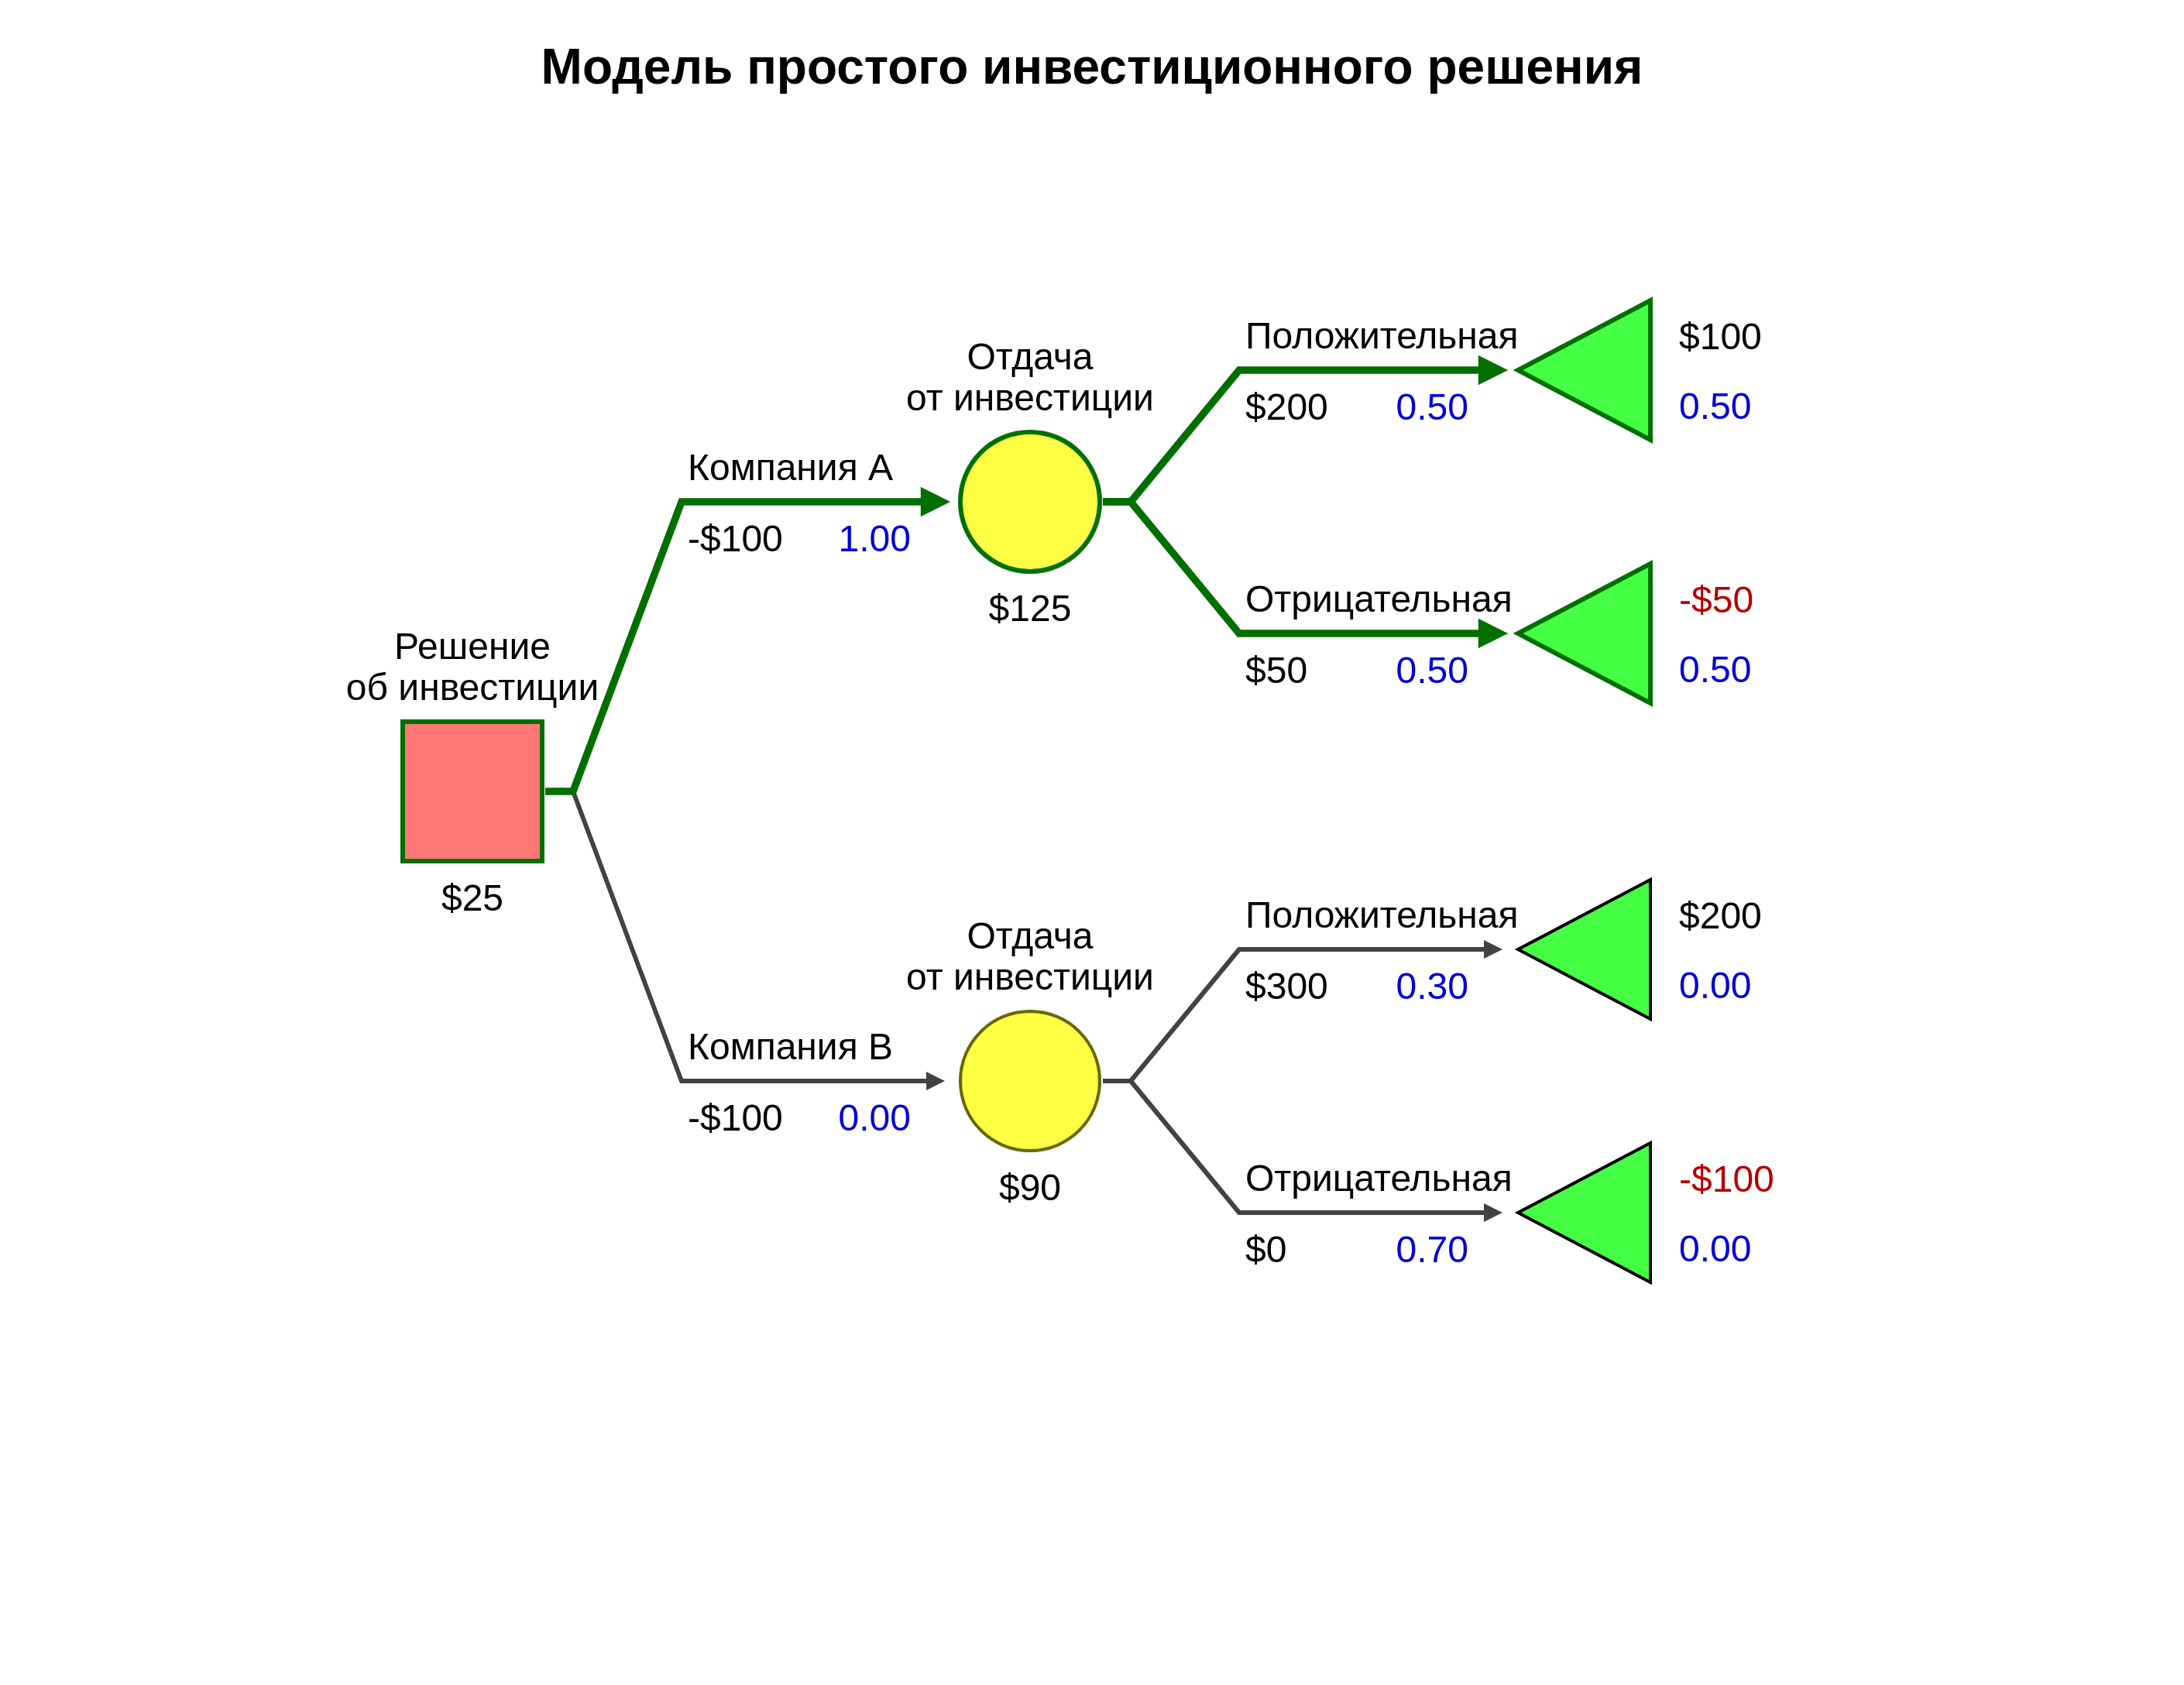
\includegraphics[width= 15cm]{pics/simple_decision_tree_1.png} 
	\label{fig:sample}
	\caption{Простое дерево решений}
\end{figure}

Модель дерева решений описывает и визуализирует последовательность принятия решения в условиях неопределенности на древовидной диаграмме. Это означает, что деревья решений могут быть полезны в таких задачах:
\begin{itemize}
    \item лицо, принимающее решение, выполняет несколько действий, следуя друг за другом,
    \item состояния мира могут различаться в зависимости от уже принятых решений,
    \item некоторые решения могут привести к более точным оценкам вероятности этих состояний.
\end{itemize}

На древовидной диаграмме представлены возможные решения, которые необходимо принять, независимые события, которые могут произойти, и результаты, связанные с комбинациями этих решений и событий. Необходимо определить два параметра: вероятности событий и их значения или стоимости. Первый параметр представляет вероятность получения определенного состояния мира. Поскольку возможные состояния мира в рамках одной реакции на самом деле являются конкурирующими событиями, сумма их вероятностей должна быть равна 1. 
Тогда значения или стоимости, выраженные в некоторой шкале, например в деньгах, означают платежи (изменение стоимости) как следствие решения или состояния мира. 
Это может быть как прибыль, так и убытки. Модель дерева решений включает еще одно понятие: EMV - ожидаемая значение или ожидаемая ценность (или ожидаемая полезность). Она вычисляется как вероятностно-взвешенное среднее значений для конкурирующих наборов решений и событий. Ожидаемое значение EMV показывает, сколько человек может заработать или потерять, принимая оптимальные решения (это означает такие решения, которые максимизируют прибыль и минимизируют убытки). Наконец, результат, связанный с решениями и событиями, представляет собой общее последствие набора решений и событий во всем процессе принятия решения. Он может быть истолкован как отдача лица, принимающего решение - результат как его решений, так и произошедших независимых событий.

Деревья решений с их простой для понимания структурой являются отличным инструментом для решения задач анализа. Они позволяют исследовать возможные результаты принятия решений и помогают выбирать между различными направлениями действий. Основной целью модели дерева решений является определение наилучшей возможной политики, которая представляет собой наибольшую отдачу или наименьший убыток.


Дерево решений строится по направленному графику слева направо, с набором узлов, которые разбиваются на три разрозненных множества:
\begin{itemize}
    \item узлы решения - типично представленные в виде квадратов,
    \item случайные узлы, представленные в виде кругов,
    \item терминальные узлы представлены в виде треугольников.
\end{itemize}

Крайняя левая вершина называется корневой вершиной и является первой вершиной принятия решения (первый красный квадрат слева - см. выше простую модель принятия инвестиционного решения - рисунок \ref{fig:sample} ). В узлах принятия решений выбирает именно тот, кто принимает решение, т.е. выбирает ровно одну из ветвей, выходящих из этого узла. Эти ветви представляют собой набор доступных альтернатив решения (действий). В случайном узле (желтые кружки - дерево образцов выше) каждая из вытекающих из него ребер - реакция - выбирается случайным образом с заданной вероятностью события. Терминальные узлы (синие треугольники на дереве выборки выше) представляют собой результат последовательности действий/реакций от корневого узла к данному конкретному терминальному узлу. Терминальный узел является конечной точкой: никакие решения не могут быть приняты, и никакие события не могут произойти после этого.

В приложении SilverDecisions вероятность событий и значения, связанные с этими событиями или решениями, определяются по краям. Ожидаемые значения, рассчитанные для каждого набора решений/событий, отображаются в каждом узле решения/шанса, а терминальные узлы показывают результаты и вероятности того, что событие окажется в указанном терминальном узле.

Обратите внимание, что каждое ребро совмещается с двумя узлами: левый, из которого выходит ребро, называется родительским узлом, а второй, находящийся справа, называется дочерним узлом. Поддерево - это еще один термин, связанный с деревьями решений - оно представляет собой ту часть дерева, которая начинается в любом дочернем узле, и каждый из них вместе с любыми потомками образует поддерево. Например, поддерево, уставившееся в корневой узел, представляет собой целое дерево.




\section{Задачи с примерами решения}
Расчеты с \url{http://silverdecisions.pl/}

Детальное описание алгоритма построения деревьев для ряда задач и набор задач для самостоятельного решения.

Можно использовать материалы из книги making good decisions.

\subsection{Исследования на разведочной скважине}
    
    
Оцените стоит ли проводить комплекс исследований на разведочной скважине со следующими параметрами:
\begin{itemize}
    \item Стоимость 1 млн руб
    \item Ожидаемая информация – фильтрационные параметры пласта, уточнение строение пласта
    \item Вероятность успешности исследования (получения какой то информации) 70%
    \item Ожидается что исследование подтвердит увеличение запасов на 15% (60% что запасы увеличатся)
    \item Текущие извлекаемые запасы – 1 млн т. нефти, стоимость 1 т.нефти в запасах – 1 тыс. руб.
\end{itemize}     
Стоит ли проводить исследование? 

    
\subsection{КВД на добывающей скважине}

Оцените стоит ли проводить КВД на эксплуатационной скважине с дебитом 50 т/нефти, Рзаб = 50 атм, Рпл = 250 атм
\begin{itemize}
    \item Стоимость исследования 1 млн руб
    \item Длительность 1 неделя (скважина остановлена)
    \item Ожидаемая информация – фильтрационные параметры пласта, скин фактор
    \item Вероятность успешности исследования (получения какой то информации) 70%
    \item Ожидается что исследование подтвердит наличие положительного скин фактора
    \begin{itemize}
        \item S=0 с вероятностью 50%
        \item S=5 с вероятностью 40%
        \item S=15 с вероятностью 10%
    \end{itemize}
    \item Стоимость кислотной обработки снижающей скин в 2 раза 1 млн руб. Длительность эффекта 1 год
    \item Стоимость нефти 1 т = 10 тыс. руб.
\end{itemize}
Стоит ли проводить исследование? 

\subsection{Исследование фонтанирующей скважины}
Имеется фонтанирующая скважина. Дебит нефти 30 т/сут. Воды нет. Имеется водоносный пласт под продуктивным. Перемычка 10 м. Вероятность получения прорыва воды после ГРП 50 \%. При прорыве воды рост обводненности до 90 \% без увеличения дебита нефти. Без прорыва воды увеличение продуктивности в 3 раза. Стоимость ГРП 1 млн. руб.

Оценить что делать на скважине?

Ничего не делать
Сделать ГРП
Провести исследование и по его результатам ГРП
Стоимость исследования 100 т.р.

Вероятность выявления скважины где ГРП будет успешен 60%